\chapter{Ambiente e strumenti}
\section{Il debugger - GDB e QEMU}
\subsection{Quick emulator - QEMU}
QEMU é un emulatore open-source, permette di emulare l'architettura di un processore. Permette quindi l'utilizzo di vari sistemi operativi ad un livello di virtualizzazzione Kernel-Based (Kernel Vitual Machine - KVM) con il beneficio di prestazioni vicine all'hardware. Per il nostro utilizzo QEMU emula un sistema x86-64. 
\subsection{GNU Debugger - GDB}
GNU Debugger (GDB) è un debugger portatile, permette quindi di testare e effettuare il debug di programmi. Eseguire il programma in questo ambiente controllato permette al programmatore di tenere traccia dell'esecuzione e monitorare le risorse al fine di individuare un eventuale malfunzionamento nel codice. Per la realizzaione dell'estensione utilizzeremo la funzione di debug remoto per connetterci ad un socket di sistema utilizzato da QEMU per il debug. GDB utilizza delle chiamate di sistema chiamate \codeword{process trace} (\codeword{ptrace}). 

\subsubsection{Breakpoints}
Un breakpoint permette al programma in esecuzione all'interno di un debugger di interrompere il flusso in un determinato punto. Si realizzano sostituendo all'istruzione, alla quale si vuole fermare l'esecuzione, una speciale istruzione la quale solitamente invia un segnale SIGTRAP, il quale verrà catturato dal debugger. Il procedimento di sostituzione è eseguito dal debugger stesso prima di avviare l'esecuzione, nel caso di GDB il programmatore deve eseguire il comando \codeword{break [arg]} dove l'argomento può essere la specifica linea di codice o un simbolo. All'interno di VSCode vi é la possibilità di inserire breakpoint cliccando sul lato sinistro della riga di codice interessata, si occuperá poi di comunicare al Debug Adapter (TODO: inserisci hyperlink a chapter del DP) la richiesta di inserimento dell'interruzione.

\begin{figure}[h]
    \centering
    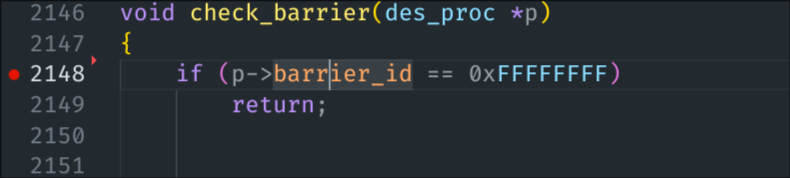
\includegraphics[width=0.7\columnwidth]{images/breakpoint_vscode.png}
    \caption{Esempio di un breakpoint in VSCode}
    \label{fig:breakpoint}
\end{figure}

\subsubsection{Continue & Stop}

\subsubsection{Step Over}

\subsubsection{Step In}

\subsubsection{Step Out}

\subsubsection{Watch delle variabili}

\subsubsection{Call Stack}

\section{L'architettura del debugger di VS Code}

\subsection{Debug Adapter - DP}

\subsection{Debug Adapter Protocol- DAP}

\subsection{Estensione CppTools}
utilizzeremo quindi un DP già realizzato dall'estensione di CppTools
\section{Webview di VS Code}

\begin{figure}[h]
    \centering
    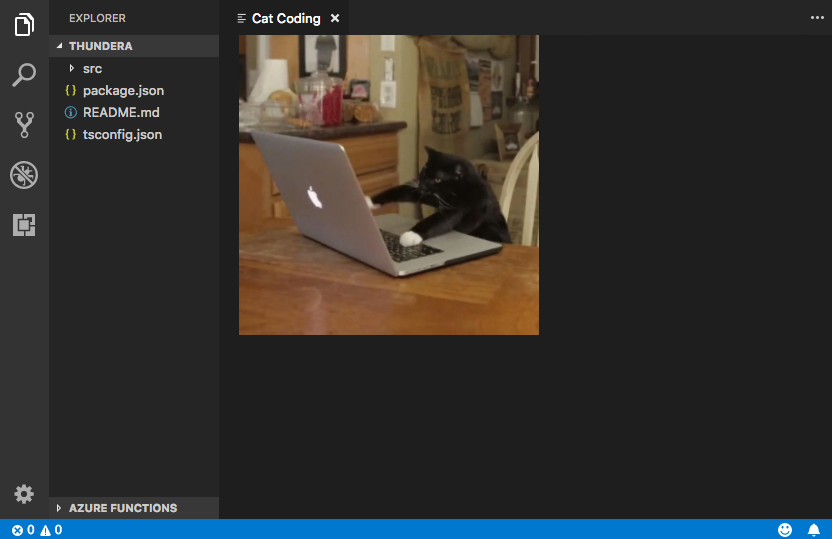
\includegraphics[width=0.7\columnwidth]{images/cat_coding.png}
    \caption{Esempio di una webview in VSCode}
    \label{fig:webcat}
\end{figure}
